\chapter{Theory}
\section{Deep neural networks}
This section introduces only the neural network parts that are used later in the thesis. The baseline model relies on dense layers, nonlinear activations, dropout, normalization, and mini batch training. The graph model also uses residual blocks, layer normalization, and a feed forward block that is used separately on each node.

\begin{figure}[htbp]
    \centering
    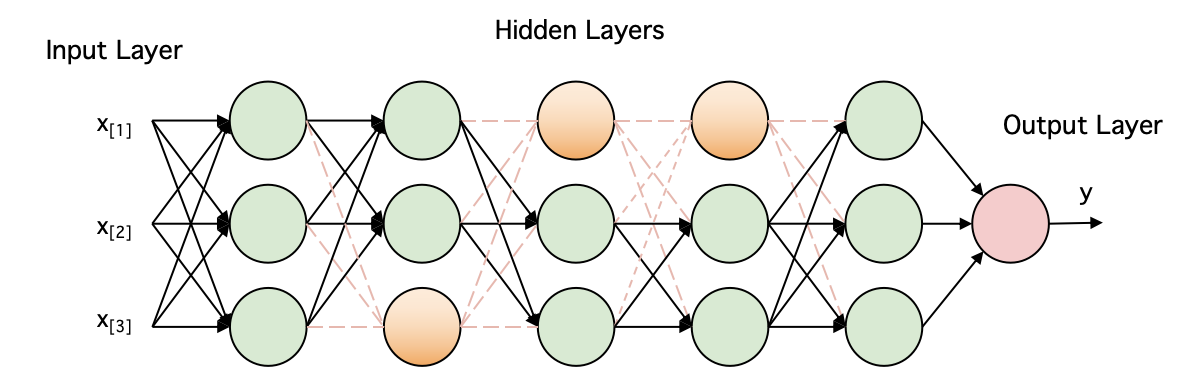
\includegraphics[width=0.95\linewidth]{figures/fully_connect_network.png}
    \caption[Feed Forward Network]{A feed forward network with several hidden layers. The circles represent units and the lines represent learned connections between layers. The highlighted orange unit is one example hidden unit, and the pink unit is the final output.}
    \label{fig:fully_connect_network}
\end{figure}

\noindent In the method figures used later, arrows show the forward flow of information. Dashed lines are used only as a visual aid. They either show omitted repeated connections or paths that are removed in one training update, depending on the figure. The symbols $W$ and $b$ always denote a weight matrix and a bias vector. In the FFN figure, $\mathrm{FFN}$ refers to the small two layer block that is applied to each node after attention. If the figure shows $N_{\mathrm{in}}$ or $N_{\mathrm{out}}$, these labels refer to the input and output feature dimensions of the displayed transformation.

\subsection{Dense layer}
A dense layer maps an input vector to a new representation:
\begin{equation}
h = \sigma(Wx + b),
\end{equation}
Here $W$ is a weight matrix, $b$ is a bias vector, and $\sigma(\cdot)$ is an activation function. Stacking dense layers lets the model transform the input step by step.

\subsection{Activation functions}
The activation function adds nonlinearity. Without it, several dense layers would still behave like one linear map. The main choice in this thesis is ReLU,
\begin{equation}
\mathrm{ReLU}(x)=\max(0,x),
\end{equation}
which is used in the dense baseline. ReLU is simple and usually works well in hidden layers. For regression tasks, the final output layer often uses no activation function.

\subsection{Stacked layers}
If $h^{(0)}=x$, a network with $L$ hidden layers can be written as
\begin{equation}
h^{(\ell+1)}=\sigma\!\left(W^{(\ell)}h^{(\ell)}+b^{(\ell)}\right), \quad \ell=0,\dots,L-1.
\end{equation}
The output of one layer becomes the input of the next, so deeper networks can build more expressive hidden representations.

\subsection{Regularization}
Regularization helps reduce overfitting and discourages solutions that are not useful for the task. In this thesis, two regularization ideas are relevant. The first is dropout, which reduces co adaptation between hidden units. The second is counterfactual regularization, which encourages the model to use drug information rather than relying too strongly on the control profile alone.

\subsubsection{Dropout}
\noindent Dropout reduces overfitting by randomly removing part of the hidden units during training~\cite{srivastava2014dropout}. If a hidden vector is $h \in \mathbb{R}^{d}$ and the dropout mask is $r \in \{0,1\}^{d}$, the dropped representation can be written as
\begin{equation}
\tilde{h}=r \odot h,
\end{equation}
\noindent where $\odot$ is element by element multiplication. If one entry of $r$ is zero, the matching hidden unit is removed in that update.

\begin{figure}[htbp]
    \centering
    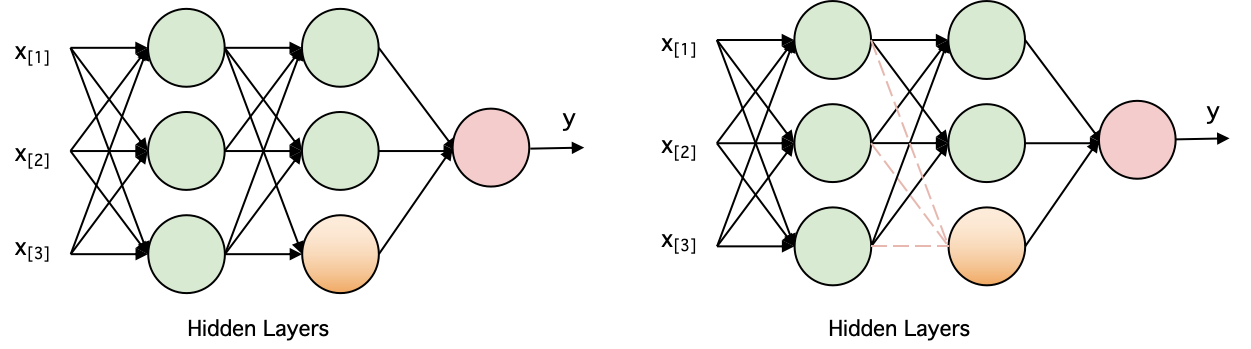
\includegraphics[width=0.95\linewidth]{figures/dropout.png}
    \caption[Dropout During Training]{Dropout during training. The left side shows the full hidden layer, while the right side shows one training update after dropout is applied. The dashed pink connections show the active paths that remain in that update. Units without a dashed incoming path are dropped for that update. The orange unit is the example target hidden unit and the pink unit is the output.}
    \label{fig:dropout}
\end{figure}

\noindent This makes the network less dependent on a small set of hidden units and often helps it work better on new data. At test time, dropout is turned off.

\subsubsection{Counterfactual regularization}
\noindent Counterfactual regularization compares two forward passes for the same sample. One pass uses the original input, and the other uses a modified version. The modified input represents a simple alternative where an important part of the input is missing or changed. That is why it is called counterfactual. If the removed or perturbed part carries useful information for the task, the original input is expected to give a better prediction than the counterfactual input.

\noindent The comparison here is simple. The model sees the same sample twice, once in its original form and once in a modified form. The training objective then encourages the model to perform better with the full input than with the modified input.

\noindent Let $\mathcal{L}_{\mathrm{full}}$ be the prediction loss from the original input and let $\mathcal{L}_{\mathrm{cf}}$ be the prediction loss from the counterfactual input. A hinge style penalty can then be written as
\begin{equation}
\mathcal{L}_{\mathrm{hinge}}=\max\!\left(0,\delta-\left(\mathcal{L}_{\mathrm{cf}}-\mathcal{L}_{\mathrm{full}}\right)\right).
\end{equation}
The training objective becomes
\begin{equation}
\mathcal{L}=\mathcal{L}_{\mathrm{full}}+\lambda_{\mathrm{cf}}\mathcal{L}_{\mathrm{hinge}}.
\end{equation}
\noindent This penalty encourages the prediction from the original input to be better than the prediction from the counterfactual input by at least a margin $\delta$~\cite{wachter2017counterfactual}. In this way, the model is discouraged from ignoring the information that was perturbed or removed. A task specific use of this idea is introduced later in the methodology chapter.

\subsection{Mini batches, learning rate, and optimizer}
During training, the full dataset is usually split into smaller groups called mini batches. Instead of using the whole dataset for every parameter update, the model uses one mini batch at a time to compute the loss and gradient. After all mini batches have been processed once, one training epoch is completed. The learning rate controls the step size of each update.

\noindent If the model parameters are written as $\theta$ and the loss on one mini batch is $\mathcal{L}_{\mathcal{B}}(\theta)$, a simple gradient based update is
\begin{equation}
\theta \leftarrow \theta - \eta \nabla_{\theta}\mathcal{L}_{\mathcal{B}}(\theta),
\end{equation}
where $\eta$ is the learning rate.

\noindent Adam is a widely used optimizer~\cite{kingma2015adam}. It combines information from past gradients and squared gradients to produce smoother parameter updates, and it is used in the experiments reported later.

\subsection{Batch and layer normalization}
Normalization helps keep hidden activations in a more stable range during training. This thesis uses two common forms, namely batch normalization and layer normalization.

\noindent Batch normalization and layer normalization use the same basic normalization form. The difference is how the mean and variance are computed. Let $a_{ij}$ denote the activation value of feature $j$ for sample $i$ in one mini batch of size $B$. In batch normalization, one mean and one variance are computed for each feature across the mini batch:
\begin{equation}
\mu_{\mathrm{batch},j}=\frac{1}{B}\sum_{i=1}^{B} a_{ij},
\qquad
\sigma_{\mathrm{batch},j}^{2}=\frac{1}{B}\sum_{i=1}^{B}(a_{ij}-\mu_{\mathrm{batch},j})^2.
\end{equation}

\noindent In layer normalization, the same idea is used, but the mean and variance are computed across the hidden features of one sample. Here $h_{ij}$ denotes feature $j$ in the hidden representation of sample $i$, and $d$ is the hidden dimension:
\begin{equation}
\mu_{\mathrm{layer},i}=\frac{1}{d}\sum_{j=1}^{d} h_{ij},
\qquad
\sigma_{\mathrm{layer},i}^{2}=\frac{1}{d}\sum_{j=1}^{d}(h_{ij}-\mu_{\mathrm{layer},i})^2.
\end{equation}

\noindent After these statistics are computed, the normalization step has the same form:
\begin{equation}
\mathrm{Norm}(x)=\gamma \frac{x-\mu}{\sqrt{\sigma^{2}+\epsilon}}+\beta.
\end{equation}
Here $\gamma$ and $\beta$ are learned scale and shift parameters, and $\epsilon$ is a small constant added to avoid division by zero. Batch normalization is used in the dense baseline, while layer normalization is used in the graph attention blocks.

\begin{figure}[htbp]
    \centering
    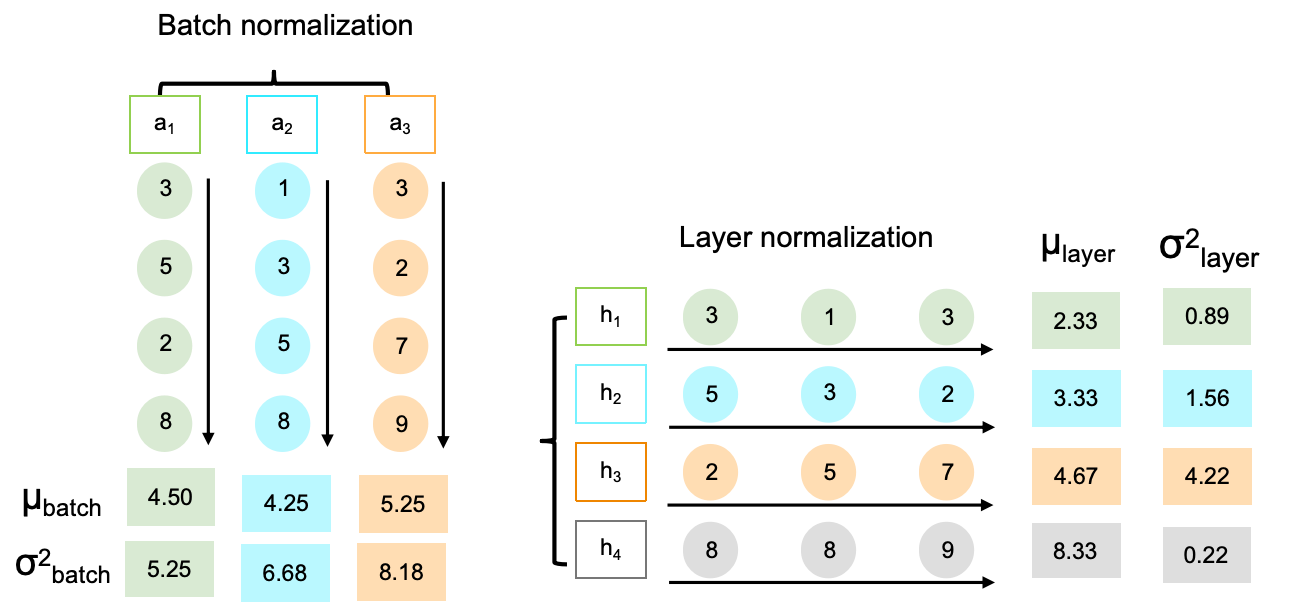
\includegraphics[width=\linewidth]{figures/BN_LN.png}
    \caption[Batch vs Layer Normalization]{Comparison of batch normalization and layer normalization. The left panel shows batch normalization, where the statistics are computed for each feature over the mini batch. The right panel shows layer normalization, where the statistics are computed over the hidden features of one sample.}
    \label{fig:bn_ln}
\end{figure}

\FloatBarrier
\section{Graph neural networks}
\subsection{Graphs}
A graph represents relations between a collection of objects. The objects are called nodes, and the relations are called edges. Mathematically, a graph is written as $G=(V,E)$, where $V$ is the set of nodes and $E$ is the set of edges. Each edge connects a pair of nodes. Figure~\ref{fig:graph_components} shows a simple directed graph.

\begin{figure}[htbp]
    \centering
    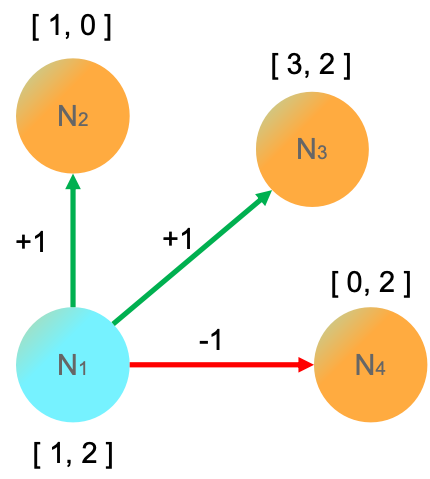
\includegraphics[width=0.369\linewidth]{figures/graph.png}
    \caption[Directed Graph Example]{Example of a directed graph. The circles are nodes, and the arrows are directed edges that show the direction of a relation from one node to another. In graph based models, nodes can also carry feature vectors and edges can carry attributes such as direction, sign, or weight.}
    \label{fig:graph_components}
\end{figure}

\noindent In this example, $N_1$, $N_2$, $N_3$, and $N_4$ are nodes. The arrows indicate that the relations have direction, so an edge from $N_1$ to $N_3$ is not the same as an edge from $N_3$ to $N_1$. In many graph learning settings, each node can additionally have its own feature vector, and each edge can also have attributes such as a sign or a weight.

\subsection{Inputs}
The input to a graph neural network is not only the graph structure. It usually includes the graph connectivity together with feature information attached to nodes, edges, or the whole graph. Let a graph have $N$ nodes. Its connectivity can be written as an adjacency matrix $A$, and the initial node feature matrix can be written as $H^{(0)}$. The pair $(A,H^{(0)})$ is the most basic input to a graph neural network.

\noindent In practice, the graph structure is often stored as an adjacency matrix. Figure~\ref{fig:graph_to_adj} shows this idea. The graph on the left is written as a matrix on the right. If there is an edge from node $N_j$ to node $N_i$, then the corresponding entry in the matrix is nonzero. If there is no edge, the entry is zero. This matrix form is convenient because the model can use it directly in message passing and neighborhood aggregation.

\begin{figure}[htbp]
    \centering
    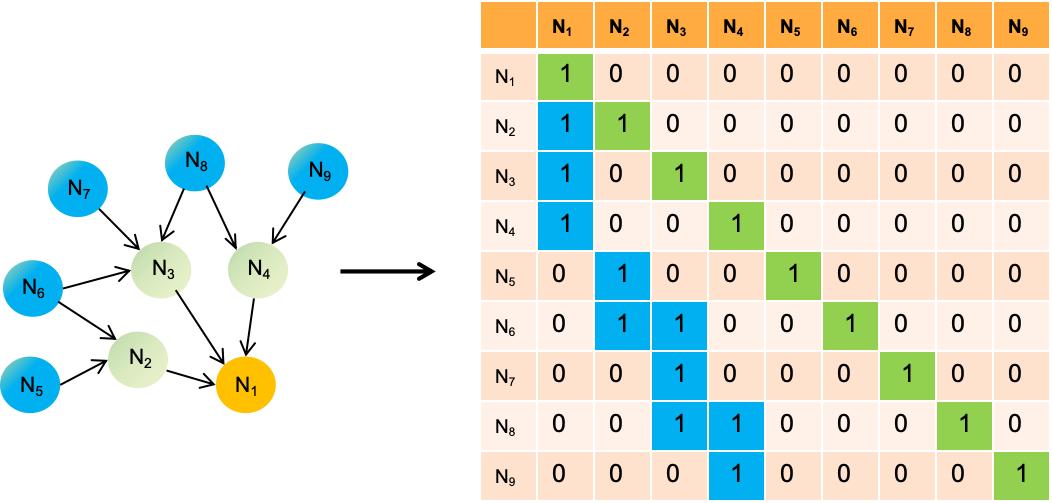
\includegraphics[width=0.8075\linewidth]{figures/graph2adj.png}
    \caption[Graph to Adjacency Matrix]{From a graph to its adjacency matrix. The graph structure is converted into a matrix form so that graph connections can be used in computation.}
    \label{fig:graph_to_adj}
\end{figure}

\noindent A node can have its own attributes, such as an expression value or a feature vector. An edge can also have attributes, such as direction, sign, or weight. Adding self loops is also common, because it lets the model keep part of the node's own state during aggregation. In biological graphs, such self loops should be understood as a model design choice rather than as a biological claim.

\subsection{Graph direction}
Graphs can be directed or undirected. In an undirected graph, the connection between two nodes has no direction. Information can move both ways. In a directed graph, each edge has a source node and a target node. So information flows from one node to another in a specific direction.

\noindent This difference matters in biology. Many molecular relations are directional. A regulator can affect a target gene, but the reverse relation may not hold. So a directed graph is often a more natural representation than an undirected graph. Once the graph structure is defined, a graph neural network still needs a rule for how information moves along these edges.

\subsection{Message passing mechanism}
This is the core idea that lets a graph neural network use the graph structure. The network works by moving data along the edges of the graph. In one layer, a node gets messages from its directly connected neighbors. For example, look at Figure~\ref{fig:gnn_message_pass_update}. Node $N_4$ collects data from its direct neighbors $N_1$, $N_2$, and $N_3$. This figure only shows what happens in one layer.

\begin{figure}[htbp]
    \centering
    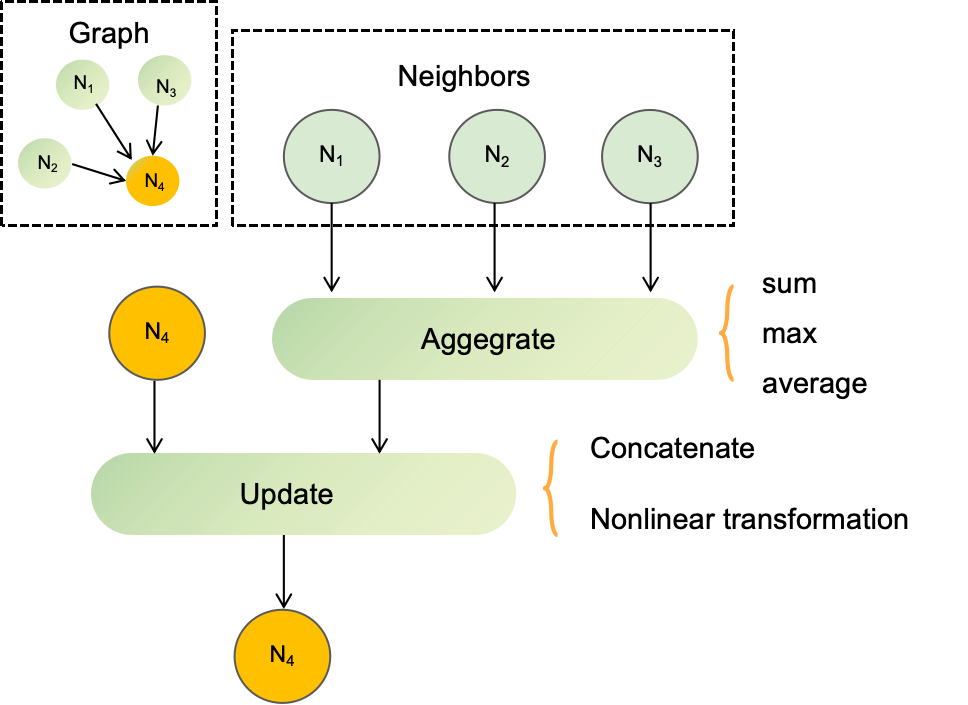
\includegraphics[width=0.646\linewidth]{figures/gnn_message_update_aggegrate.png}
    \caption[Single Layer Message Passing]{Message passing in a single layer. Messages from neighbors are grouped together and then used to update the target node.}
    \label{fig:gnn_message_pass_update}
\end{figure}

\noindent After one layer, a node holds information from its direct neighbors. When more layers are stacked, the receptive field becomes larger and the node can also receive information from more distant parts of the graph.

\begin{figure}[htbp]
    \centering
    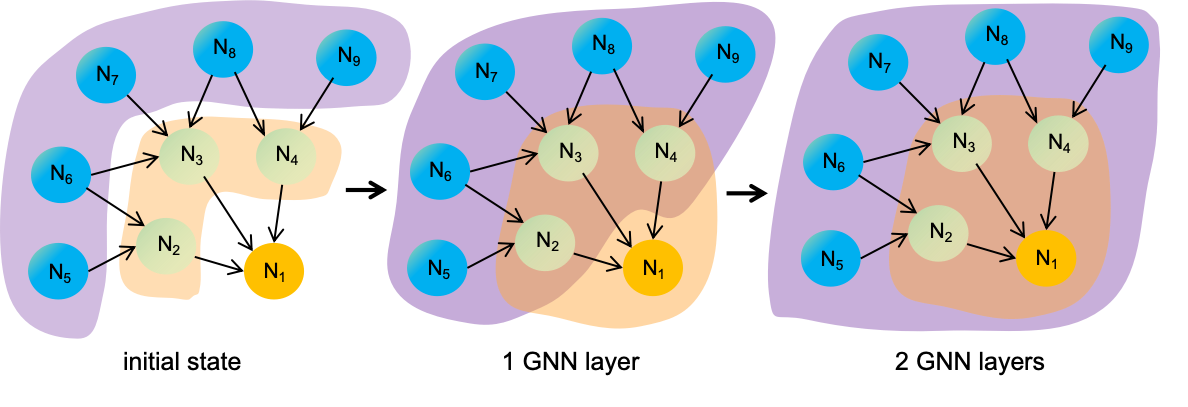
\includegraphics[width=0.95\linewidth]{figures/2_layers_message_passing.png}
    \caption[Two Layer Message Passing]{How message passing expands across layers. The yellow node $N_1$ is the target node. After one layer, it receives information from its one hop neighbors $N_2$, $N_3$, and $N_4$. After two layers, information from the two hop neighbors $N_5$ to $N_9$ can also reach $N_1$ through the intermediate nodes.}
    \label{fig:two_layer_message_passing}
\end{figure}

\noindent Figure~\ref{fig:two_layer_message_passing} shows this idea. In the first layer, node $N_1$ only uses the states of its one hop neighbors. In the second layer, those neighbors already contain information from nodes that are two hops away. This is why stacking local message passing layers still expands the effective range of information flow.

\noindent Message passing can be separated into two steps. Aggregation groups the incoming neighbor signals, and update uses the grouped message to compute a new node state.

\subsubsection{Aggregation}
The first step is aggregation. In this step, node $v$ collects the messages sent by its neighbors and turns them into one summary vector. Here, $\mathcal{N}(v)$ denotes the set of neighbors that send messages to node $v$. In a directed graph, these are the incoming neighbors of $v$. A common way to write this step is
\begin{equation}
m_{\mathcal{N}(v)}^{(\ell)} = \mathrm{Agg}^{(\ell)}\!\left(\left\{m_{u \rightarrow v}^{(\ell)} \mid u \in \mathcal{N}(v)\right\}\right),
\end{equation}
Here, $m_{u \rightarrow v}^{(\ell)}$ is the message sent from neighbor $u$ to node $v$ at layer $\ell$. The braces indicate that aggregation uses the full set of incoming messages as input. The symbol $\mathrm{Agg}^{(\ell)}$ stands for the aggregation function that combines these messages into one summary vector. Common choices for $\mathrm{Agg}^{(\ell)}$ are sum, mean, and max.

\noindent The neighbors of a node do not come in a natural left to right order. For this reason, the summary should stay the same even if the neighbors are listed in a different order.

\subsubsection{Update}
The second step is update. After the neighbor messages have been summarized, the node combines this summary with its current state and produces a new state. An update at layer $\ell$ uses a learned function $\psi^{(\ell)}$:
\begin{equation}
h_{v}^{(\ell+1)} = \psi^{(\ell)}\!\left(h_{v}^{(\ell)}, m_{\mathcal{N}(v)}^{(\ell)}\right),
\end{equation}
Here, $h_{v}^{(\ell)}$ is the state of node $v$ at layer $\ell$, and $h_{v}^{(\ell+1)}$ is the updated state at the next layer. The role of $\psi^{(\ell)}$ is to decide how the node should change after receiving the summarized neighbor message. This is different from the aggregation step itself. Aggregation combines neighbor messages, while the update step changes the node state.

\noindent The update function is the step that actually changes the node state. In a mini batch, the graph structure stays the same for all samples. The model repeats these aggregation and update steps for several layers. After that, it gets the final node states.

\noindent The final node representation matrix is denoted by $H^{(L)}$. What happens next depends on the output form of the model.

\subsection{Output}
Graph neural networks can produce several kinds of outputs. One common choice is one prediction for each node. This is used in node classification and node regression. Another choice is one prediction for a pair of nodes or for an existing edge. This is common in link prediction and edge classification. A third choice is one prediction for the whole graph. This is often used in graph classification or graph regression.

\begin{figure}[!t]
    \centering
    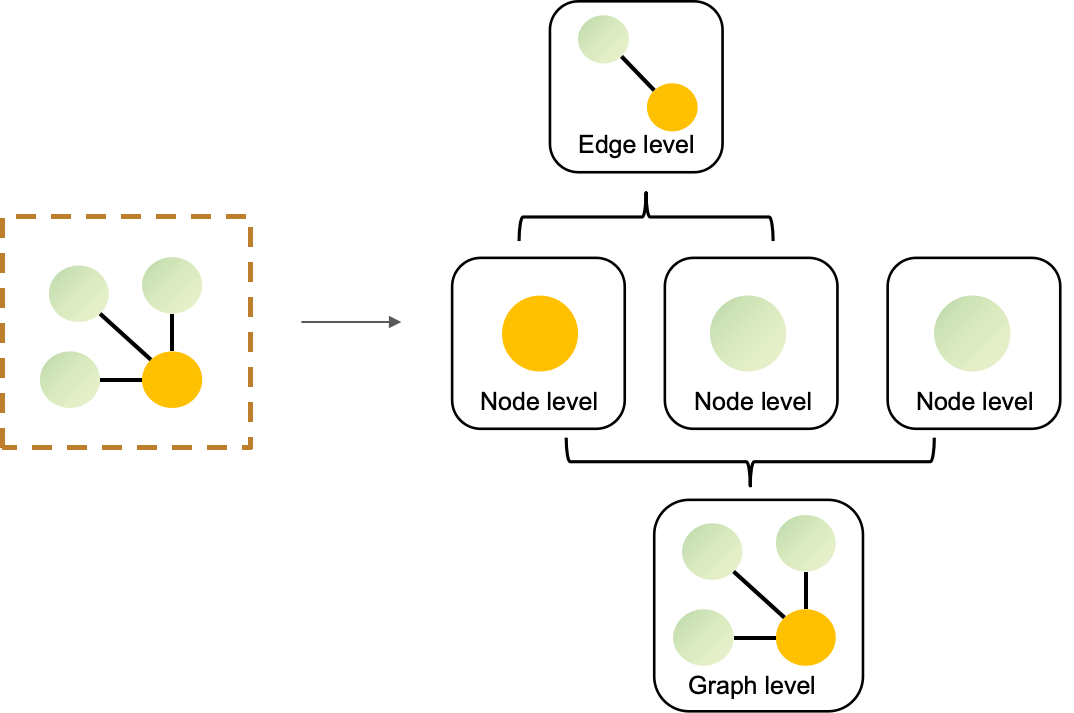
\includegraphics[width=0.64\linewidth]{figures/gnn_output.png}
    \caption[GNN Output Types]{Three common GNN output types. A GNN can produce one output for each node, one output for a selected edge, or one output for the whole graph after a readout step.}
    \label{fig:gnn_output}
\end{figure}

\noindent The output type determines how the final hidden states are used. If the model predicts one value for each node, it applies a predictor to each row of $H^{(L)}$. If the model predicts one value for an edge, it combines the representations of two nodes, and sometimes also an edge feature, to predict a relation between them. If the model predicts one value for the whole graph, it must reduce all node representations to one graph representation before the final prediction.

\noindent This reduction step is usually called pooling or readout. Common choices are sum pooling, mean pooling, and max pooling. Sum pooling adds node vectors and can reflect graph size. Mean pooling gives a more normalized summary. Max pooling keeps the strongest value in each feature dimension. Some models also use attention based pooling, where the model learns which nodes should contribute more to the graph representation.

\noindent The output type is related to the final task, but the task itself can still vary within the same setting. For example, predictions for each node can be used for either classification or regression. Predictions for the whole graph can also be used for either classification or regression. In this thesis, the model predicts a continuous drug response value for each gene. Each gene is treated as a node in the biological graph. So the thesis predicts one continuous value for each node.

\subsection{Graph Attention Networks (GAT)}
Graph Attention Networks (GATs) give different weights to different neighbours~\cite{velickovic2018graph}. Figure~\ref{fig:attention_mechanism} shows how the attention weights are computed.

\begin{figure}[htbp]
    \centering
    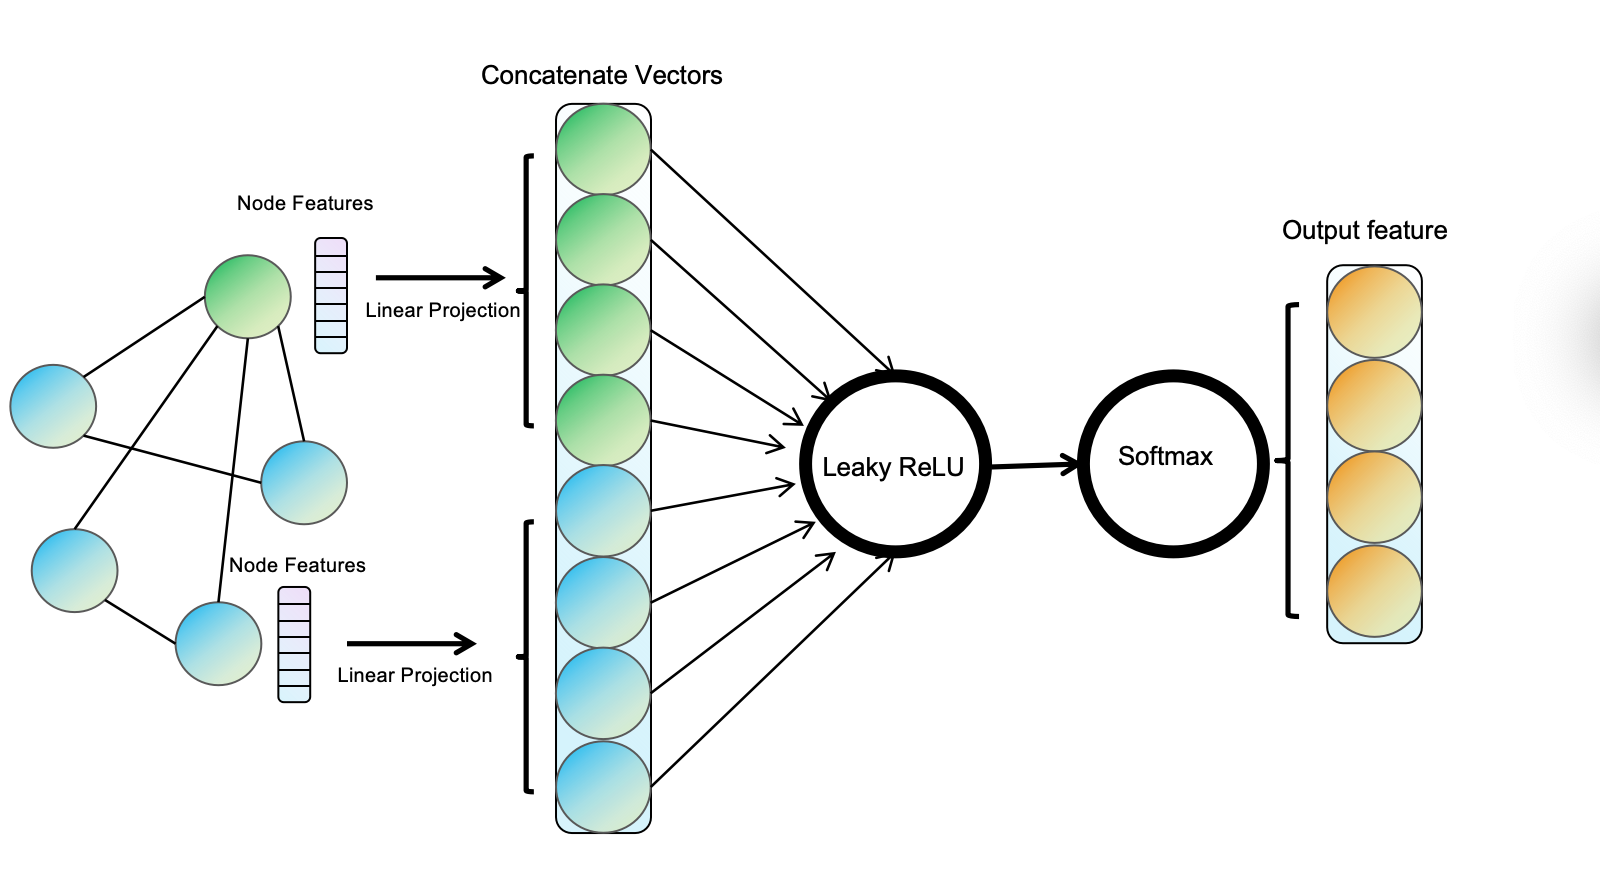
\includegraphics[width=0.95\linewidth]{figures/attention_mechnisam.png}
    \caption[GAT Attention Scores]{Computation of attention scores and normalized attention weights in a graph attention layer. The left side shows source and target node features. The middle stacked vectors show their linear projections and concatenation. The arrows show the computation path from projection to score, from score to softmax, and then to the normalized output feature.}
    \label{fig:attention_mechanism}
\end{figure}

\noindent GAT differs from GCN because it does not use one fixed normalized weighting rule for all neighbours. Instead, it learns how important each neighbour is for the current target node. This makes the aggregation more flexible.

\subsubsection{GAT layer}
\noindent Let $h_{u}^{(\ell)}$ and $h_{v}^{(\ell)}$ be node representations at layer $\ell$. A GAT layer first applies a learned projection
\begin{equation}
z_{u}^{(\ell)} = W^{(\ell)} h_{u}^{(\ell)},
\end{equation}
Here $W^{(\ell)}$ is a learned projection matrix. It then computes an attention score
\begin{equation}
e_{u \rightarrow v}=\mathrm{LeakyReLU}\!\left(a^{\top}\left[z_{u}^{(\ell)} \Vert z_{v}^{(\ell)}\right]\right),
\end{equation}
Here $a$ is a learned vector, and $\Vert$ denotes concatenation of the two projected node vectors. The LeakyReLU function is
\begin{equation}
\mathrm{LeakyReLU}(x)=
\begin{cases}
x, & x \ge 0, \\
\alpha x, & x < 0,
\end{cases}
\end{equation}
Here $\alpha$ is a small positive constant. The normalized attention weight is
\begin{equation}
\alpha_{u \rightarrow v}=
\frac{\exp(e_{u \rightarrow v})}
{\sum_{u' \in \mathcal{N}(v)} \exp(e_{u' \rightarrow v})}.
\end{equation}
This normalization is carried out over all neighbors that send messages to node $v$. If the graph layer includes a self loop, then node $v$ is also included in $\mathcal{N}(v)$.
The new node representation is
\begin{equation}
h_{v}^{(\ell+1)}=\sigma\!\left(\sum_{u \in \mathcal{N}(v)} \alpha_{u \rightarrow v} z_{u}^{(\ell)}\right).
\end{equation}

\noindent These attention weights are learned from data. They depend on the features of both the source node and the target node, so the same neighbour can receive different importance in different local settings.

\subsubsection{Multi-head attention}
\noindent GAT can also use several attention heads in parallel. If the model uses $K$ heads, each head has its own projection and attention parameters. The outputs can be concatenated or averaged, depending on the layer design.

\noindent If each head outputs $F_{\mathrm{head}}$ features and the model concatenates the heads, then the output width is
\begin{equation}
F_{\ell+1}=K F_{\mathrm{head}}.
\end{equation}
This relation is useful when model dimensions are chosen in practice.

\noindent Multi head attention gives the model several views of the same neighborhood and can make the representation richer than using one attention rule alone.

\subsubsection{Residual connections}
Residual connections add the input of a block back to its output~\cite{he2016residual}. If a block computes a transformation $f(x)$, the residual form returns
\begin{equation}
z=x+f(x).
\end{equation}
Figure~\ref{fig:residual_connections} shows this idea. The input $x$ goes through the stacked layers and also follows a shortcut path. These two paths are added at the end.

\begin{figure}[htbp]
    \centering
    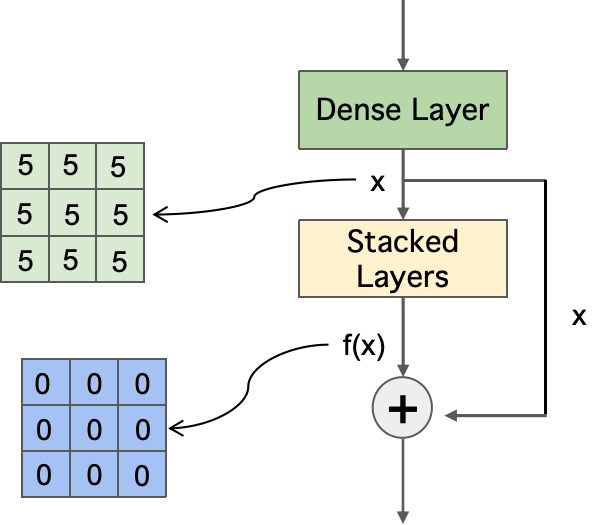
\includegraphics[width=0.4455\linewidth]{figures/resNet.png}
    \caption[Residual Connection]{A residual connection. The input follows both the main stacked layers and a shortcut path, and the two outputs are added together.}
    \label{fig:residual_connections}
\end{figure}

\noindent This design keeps a direct path from the input to the output of the block. It helps preserve useful information from earlier layers and often makes optimization more stable in deeper models.

\subsubsection{Feed forward network after attention}
In Transformer related models, an attention layer is often followed by a small two layer block, often called an FFN~\cite{vaswani2017attention}. In this thesis, the term FFN in this part always refers to that small block after attention, not to the full feed forward network shown earlier in the chapter.

\begin{figure}[htbp]
    \centering
    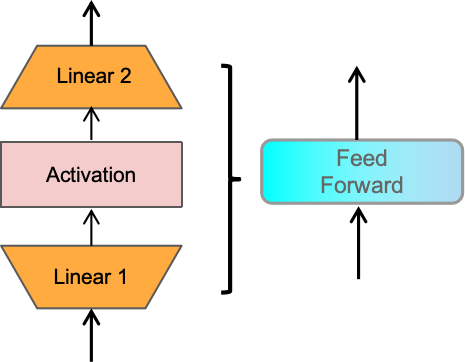
\includegraphics[width=0.715\linewidth]{figures/FFN.png}
    \caption[FFN Block]{A small two layer block applied to each node representation after attention. The input vector is transformed by a first affine map with parameters $W_{1}$ and $b_{1}$, then passed through a nonlinear activation, and then mapped back by a second affine map with parameters $W_{2}$ and $b_{2}$. If the figure shows $N_{\mathrm{in}}$ and $N_{\mathrm{out}}$, they indicate the input width and the hidden width of this block. The arrows show the forward data flow.}
    \label{fig:ffn_block}
\end{figure}

\noindent Figure~\ref{fig:ffn_block} shows the structure of this block. It applies two linear layers to the input node state with an activation function in between. If the node state after attention is $h_{v}$, the model computes the FFN output like this:
\begin{equation}
\label{eq:ffn_block}
\mathrm{FFN}(h_{v}) = W_{2}\,\sigma(W_{1}h_{v}+b_{1})+b_{2}.
\end{equation}
Here $W_{1}$ and $W_{2}$ are the weight matrices and $b_{1}, b_{2}$ are the bias vectors. The first linear layer expands the feature dimension from $d_{\mathrm{model}}$ to a larger dimension $d_{\mathrm{ff}}$, and the second projects it back to $d_{\mathrm{model}}$. In the schematic figure, $N_{\mathrm{in}}$ corresponds to $d_{\mathrm{model}}$ and $N_{\mathrm{out}}$ corresponds to $d_{\mathrm{ff}}$. The same parameters are shared across all nodes, and the same block is used for each node.

\subsubsection{GAT attention block}
\noindent In the original GAT definition, the core operation is the attention based neighborhood aggregation described above~\cite{velickovic2018graph}. In many later attention based models, the attention layer is followed by the small two layer block described above, with residual connections and layer normalization around these sublayers~\cite{vaswani2017attention,he2016residual,ba2016layernorm}. This design became widely known through the Transformer architecture~\cite{vaswani2017attention} and was later adopted in graph Transformer style models such as Graphormer and GraphGPS~\cite{ying2021graphormer,rampasek2022graphgps}.

\noindent Each part in this block has a different role. Attention mixes information across neighboring nodes, the FFN further transforms each node representation, residual connections preserve useful earlier information, and layer normalization helps keep training stable~\cite{vaswani2017attention,he2016residual,ba2016layernorm}. This design was later adopted in graph Transformer style models such as Graphormer and GraphGPS~\cite{ying2021graphormer,rampasek2022graphgps}.
\subsubsection{Advantage}
\noindent GAT can be more useful when the graph is noisy or incomplete. In many real datasets, some edges are weak, indirect, or uncertain. A fixed aggregation rule treats all neighbours in a similar way after normalization. Attention can reduce the influence of less informative neighbours and give more weight to neighbours that appear more relevant for the current prediction. This does not remove graph noise, but it can make the model more robust to it.

\subsection{Uncertainty estimation}

\noindent Predictions should not always be interpreted as equally reliable. Uncertainty estimation is used to represent this difference. Instead of giving only one predicted value, the model can also describe how certain or uncertain that prediction is. In this thesis, the uncertainty mainly refers to input dependent noise in the prediction target rather than uncertainty in the model parameters.

\subsubsection{Gaussian assumption}
\noindent A regression target does not need to be treated as one fixed value only. It can also be modeled as a random variable with a conditional probability distribution. In probabilistic regression, a common assumption for a continuous target is a Gaussian likelihood whose mean and variance depend on the input~\cite{bishop2006pattern,kendall2017uncertainties}. In this thesis, the conditional target distribution is written as
\begin{equation}
\label{eq:gaussian_assumption}
y \mid x \sim \mathcal{N}\!\left(\mu(x),\sigma^{2}(x)\right).
\end{equation}
Here $\mu(x)$ is the input dependent mean and $\sigma^{2}(x)$ is the input dependent variance. A small variance means that the target is expected to stay close to the mean, while a large variance means that the prediction is treated as less certain.

\noindent This thesis does not strictly prove that the conditional target distribution is Gaussian. The Gaussian likelihood is used as a practical modeling assumption for probabilistic regression. Its reasonableness is instead assessed empirically through test negative log likelihood, residual diagnostics, and coverage analysis of the prediction bands.

\subsubsection{Predicting mean and variance}
\noindent Under this view, the model predicts two values instead of one. The first is the mean prediction $\mu$, and the second is a variance related term. In practice, models often predict $\log \sigma^{2}$ instead of $\sigma^{2}$ directly, because this is easier to train, more stable, and still defines a positive variance after exponential operation~\cite{kendall2017uncertainties}.

\subsubsection{Negative log likelihood}
\noindent If the target is modeled with a Gaussian distribution, a natural training objective is the negative log likelihood (NLL). its general form is
\begin{equation}
\label{eq:gaussian_nll}
\mathcal{L}_{\mathrm{NLL}}=\frac{1}{2}\left[\log \sigma^{2}+\frac{(y-\mu)^{2}}{\sigma^{2}}\right].
\end{equation}
The squared error term encourages the mean prediction to stay close to the target. The $\log \sigma^{2}$ term penalizes unnecessarily large uncertainty. Together, these two terms prevent the model from assigning high variance everywhere while still allowing uncertain predictions when needed.

\subsubsection{Summary}
\noindent Uncertainty estimation is useful when some targets are easier to predict than others. In biological data, some responses are clearer and more consistent, while others are noisier or more context dependent. Predicting both a mean and an uncertainty lets the model represent different confidence levels across genes or samples instead of treating all predictions as equally certain.
